% (c) 2017 Daniele Zambelli - daniele.zambelli@gmail.com
% 
% Tutti i grafici per il capitolo relativo alle disequazioni di secondo grado
%

\newcommand{\asseretta}[5]{% asse x e retta
  \def \lung{#1}
  \def \zero{#2}
  \def \segnoa{#3}
  \def \segnob{#4}
  \def \emme{#5}
  \disegno{      
    \assex{-\lung / 2}{+\lung / 2}{0}
    \tkzInit[xmin=-5,xmax=+5,ymin=-1.3,ymax=+1.3]
    \tkzFct[domain=-5:5,thick,color=Maroon!50!black]{\emme*x};
    \foreach \x in {-3, -1} 
      \node at (\x, 0) [above, yshift=-3pt] {\(\segnoa\)};
    \foreach \x in {1, 3} 
      \node at (\x, 0) [above, yshift=-3pt] {\(\segnob\)};
    \draw[fill=orange] (0,0) circle (1.5pt) node[below] {\(\zero\)};
  }
}

\newcommand{\rettammi}[2]{% retta m<0
  \asseretta{#1}{#2}{+}{-}{-.5}
}

\newcommand{\rettamma}[2]{% retta m>0
  \asseretta{#1}{#2}{-}{+}{+.5}
}

\newcommand{\parabolaamidmi}{% Parabola a<0 e Delta<0
  \disegno{      
    \assex{-5}{+5}{0}
    \tkzInit[xmin=-5,xmax=+5,ymin=-1.3,ymax=+1.3]
    \tkzFct[domain=-5:5,thick,color=Maroon!50!black]{-.125*x*x-.5};
    \foreach \x in {-4,...,4}
      \node at (\x, 0) [above, yshift=-3pt] {\(-\)};
  }
}

\newcommand{\parabolaamidz}[1]{% Parabola a<0 e Delta=0
  \def \zero{#1}
  \disegno{      
    \assex{-5}{+5}{0}
    \tkzInit[xmin=-5,xmax=+5,ymin=-1.3,ymax=+1.3]
    \tkzFct[domain=-5:5,thick,color=Maroon!50!black]{-.125*x*x};
    \foreach \x in {-4, -2, 2, 4} 
      \node at (\x, 0) [above, yshift=-3pt] {\(-\)};
    \draw[fill=orange] (0,0) circle (1.5pt) node[below] {\(\zero\)};
  }
}

\newcommand{\parabolaamidma}[2]{% Parabola a<0 e Delta>0
  \def \zeroa{#1}
  \def \zerob{#2}
  \disegno{      
    \assex{-5}{+5}{0}
    \tkzInit[xmin=-5,xmax=+5,ymin=-1.3,ymax=+1.3]
    \tkzFct[domain=-5:5,thick,color=Maroon!50!black]{-.25*x*x+1};
    \foreach \x in {-3, +3} 
      \node at (\x, 0) [above, yshift=-3pt] {\(-\)};
    \node at (0, 0) [above, yshift=-3pt] {\(+\)};
    \draw[fill=orange] (-2,0) circle (1.5pt) node[below] {\(\zeroa\)};
    \draw[fill=orange] (+2,0) circle (1.5pt) node[below] {\(\zerob\)};
  }
}

\newcommand{\parabolaamadmi}{% Parabola a>0 e Delta<0
  \disegno{      
    \assex{-5}{+5}{0}
    \tkzInit[xmin=-5,xmax=+5,ymin=-1.3,ymax=+1.3]
    \tkzFct[domain=-5:5,thick,color=Maroon!50!black]{+.125*x*x+.5};
    \foreach \x in {-4,...,4}
      \node at (\x, 0) [above, yshift=-3pt] {\(+\)};
  }
}

\newcommand{\parabolaamadz}[1]{% Parabola a>0 e Delta=0
  \def \zero{#1}
  \disegno{      
    \assex{-5}{+5}{0}
    \tkzInit[xmin=-5,xmax=+5,ymin=-1.3,ymax=+1.3]
    \tkzFct[domain=-5:5,thick,color=Maroon!50!black]{+.125*x*x};
    \foreach \x in {-4, -2, 2, 4} 
      \node at (\x, 0) [above, yshift=-3pt] {\(+\)};
    \draw[fill=orange] (0,0) circle (1.5pt) node[below] {\(\zero\)};
  }
}

\newcommand{\parabolaamadma}[2]{% Parabola a>0 e Delta>0
  \def \zeroa{#1}
  \def \zerob{#2}
  \disegno{      
    \assex{-5}{+5}{0}
    \tkzInit[xmin=-5,xmax=+5,ymin=-1.3,ymax=+1.3]
    \tkzFct[domain=-5:5,thick,color=Maroon!50!black]{+.25*x*x-1};
    \foreach \x in {-3, +3} 
      \node at (\x, 0) [above, yshift=-3] {\(+\)};
    \node at (0, 0) [above, yshift=-3pt] {\(-\)};
    \draw[fill=orange] (-2,0) circle (1.5pt) node[below] {\(\zeroa\)};
    \draw[fill=orange] (+2,0) circle (1.5pt) node[below] {\(\zerob\)};
  }
}

% \newcommand{\parabola}{% Parabola con intersezioni asse x.
%   \disegno{      
%     \rcom{-2}{+4}{-4}{+2}{gray!50, very thin, step=1}
%     \tkzInit[xmin=-2.3,xmax=+4.3,ymin=-4.3,ymax=+2.3]
%     \tkzFct[domain=-2.3:4.3,thick,color=Maroon!50!black]{x*x-2*x-3};
%     \draw[fill=orange] (-1,0) circle (1.5pt) 
%          node[above right] at (-1,0) {$A$};
%     \draw[fill=orange] (3,0)circle (1.5pt)
%          node[above right] at (3,0) {$B$};
% 
%   }
% }
% 
% \newcommand{\parabolaa}{% Intersezioni distinte
%   \disegno{      
%     \assecontrattini{-3}{+3}{0}{x}
%     \tkzInit[xmin=-3,xmax=+2,ymin=-4.3,ymax=+2.3]
%     \tkzFct[domain=-3:3,thick,color=Maroon!50!black]{x*x+x-2};
%     \draw[fill=orange] (-2,0) circle (1.5pt) 
%          node[below left] at (-2,0) {$-2$};
%     \draw[fill=orange] (1,0)circle (1.5pt)
%          node[below right] at (1,0) {$1$};
%   }
% }
% 
% \newcommand{\parabolab}{% Intersezioni coincidenti
%   \disegno{      
%     \assecontrattini{-1}{+5}{0}{x}
%     \tkzInit[xmin=-1,xmax=+5,ymin=-4.3,ymax=+2.3]
%     \tkzFct[domain=-1:5,thick,color=Maroon!50!black]{x*x-4*x+4};
%     \draw[fill=orange] (2,0) circle (1.5pt) 
%          node[below] at (2,0) {$2$};
%   }
% }
% 
% \newcommand{\parabolac}{% Intersezioni immaginarie
%   \disegno{      
%     \assecontrattini{-1}{+5}{0}{x}
%     \tkzInit[xmin=-1,xmax=+5,ymin=-4.3,ymax=+2.3]
%     \tkzFct[domain=-1:5,thick,color=Maroon!50!black]{x*x-4*x+4.5};
%   }
% }

% \newcommand{\intiaa}[3]{% Intervallo ]a; b[
%   \def \lung{#1}
%   \def \zeroa{#2}
%   \def \zerob{#3}
%   \disegno{
%     \coordinate (a) at (-\lung / 4.5, 0);
%     \coordinate (b) at (+\lung / 4.5, 0);
%     \assex{-\lung / 2}{+\lung / 2}{0}
%     \draw [blue, thick, decorate, decoration=snake] (a) -- (b);
%     \draw[fill=white] (a) circle (2pt) node [above] {\(\zeroa\)};
%     \draw[fill=white] (b) circle (2pt) node [above] {\(\zerob\)};
%   }
% }

\newcommand{\inti}[5]{% Intervallo interno
  \def \lung{#1}
  \def \zeroa{#2}
  \def \zerob{#3}
  \def \inta{#4}
  \def \intb{#5}
  \disegno{
    \coordinate (a) at (-\lung / 4.5, 0);
    \coordinate (b) at (+\lung / 4.5, 0);
    \assex{-\lung / 2}{+\lung / 2}{0}
    \draw [blue, thick, decorate, decoration=snake] (a) -- (b);
    \draw[fill=\inta] (a) circle (2pt) node [above] {\(\zeroa\)};
    \draw[fill=\intb] (b) circle (2pt) node [above] {\(\zerob\)};
  }
}

\newcommand{\inte}[5]{% Intervallo interno
  \def \lung{#1}
  \def \zeroa{#2}
  \def \zerob{#3}
  \def \inta{#4}
  \def \intb{#5}
  \disegno{
    \coordinate (a) at (-\lung / 4.5, 0);
    \coordinate (b) at (+\lung / 4.5, 0);
    \assex{-\lung / 2}{+\lung / 2}{0}
    \draw [blue, thick, decorate, decoration=snake] (-\lung / 2, 0) -- (a);
    \draw [blue, thick, decorate, decoration=snake] (b) -- (+\lung / 2, 0);
    \draw[fill=\inta] (a) circle (2pt) node [above] {\(\zeroa\)};
    \draw[fill=\intb] (b) circle (2pt) node [above] {\(\zerob\)};
  }
}

\newcommand{\intpunto}[3]{% Intervallo interno
  \def \lung{#1}
  \def \zerop{#2}
  \def \intp{#3}
  \disegno{
    \assex{-\lung / 2}{+\lung / 2}{0}
    \draw[fill=\intp] (0, 0) circle (2pt) node [above] {\(\zerop\)};
  }
}

\newcommand{\intiaa}[3]{% Intervallo ]a; b[
  \inti{#1}{#2}{#3}{white}{white}
}

\newcommand{\intica}[3]{% Intervallo [a; b[
  \inti{#1}{#2}{#3}{black}{white}
}

\newcommand{\intiac}[3]{% Intervallo ]a; b]
  \inti{#1}{#2}{#3}{white}{black}
}

\newcommand{\inticc}[3]{% Intervallo [a; b]
  \inti{#1}{#2}{#3}{black}{black}
}

\newcommand{\inteaa}[3]{% Intervallo ]a; b[
  \inte{#1}{#2}{#3}{white}{white}
}

\newcommand{\inteca}[3]{% Intervallo [a; b[
  \inte{#1}{#2}{#3}{black}{white}
}

\newcommand{\inteac}[3]{% Intervallo ]a; b]
  \inte{#1}{#2}{#3}{white}{black}
}

\newcommand{\intecc}[3]{% Intervallo [a; b]
  \inte{#1}{#2}{#3}{black}{black}
}

\newcommand{\puntoa}[2]{% Intervallo ]a; b[
  \intpunto{#1}{#2}{white}
}

\newcommand{\puntoc}[2]{% Intervallo [a; a]
  \intpunto{#1}{#2}{black}
}

\newcommand{\intv}[1]{% Intervallo vuoto
  \def \lung{#1}
  \disegno{
    \assex{-\lung / 2}{+\lung / 2}{0}
  }
}

\newcommand{\intr}[1]{% Intervallo vuoto
  \def \lung{#1}
  \disegno{
    \assex{-\lung / 2}{+\lung / 2}{0}
    \draw [blue, thick, decorate, decoration=snake] 
          (-\lung / 2, 0) -- (+\lung / 2, 0);
  }
}

\newcommand{\segnoprodotto}{% Segno del prodotto di due funzioni
  \disegno{
    \trespolosegni{5}{1.2}{3}{3}
  }
}

% (c) 2014 Daniele Zambelli - daniele.zambelli@gmail.com

\begin{comment}
%%%
% Studio dei segni di un prodotto
%%%%
 
\begin{tikzpicture}[x=2.5mm, y=5mm, smooth]

\coordinate (a_top) at (-5, 1);
\coordinate (a_bottom) at (-5, -3);
\coordinate (b_top) at (0, 1);
\coordinate (b_bottom) at (0, -3);
\coordinate (c_top) at (5, 1);
\coordinate (c_bottom) at (5, -3);

% (c) 2014 Daniele Zambelli - daniele.zambelli@gmail.com

%%%
% Grafo per il calcolo del segno con tre assi
%%%%
 
% (c) 2014 Daniele Zambelli - daniele.zambelli@gmail.com

%%%
% Asse cartesiano x
%%%%

% (c) 2014 Daniele Zambelli - daniele.zambelli@gmail.com

%%%
% Asse cartesiano generico
%%%%

\draw [-{Stealth[length=2mm, open, round]}] (-10, 0) -- (10, 0);

\node [below] at (10, 0)  {$x$};

\begin{scope}[yshift= -.5cm]
  % (c) 2014 Daniele Zambelli - daniele.zambelli@gmail.com

%%%
% Asse cartesiano x
%%%%

% (c) 2014 Daniele Zambelli - daniele.zambelli@gmail.com

%%%
% Asse cartesiano generico
%%%%

\draw [-{Stealth[length=2mm, open, round]}] (-10, 0) -- (10, 0);

\node [below] at (10, 0)  {$x$};

  \begin{scope}[yshift= -.5cm]
    % (c) 2014 Daniele Zambelli - daniele.zambelli@gmail.com

%%%
% Asse cartesiano x
%%%%

% (c) 2014 Daniele Zambelli - daniele.zambelli@gmail.com

%%%
% Asse cartesiano generico
%%%%

\draw [-{Stealth[length=2mm, open, round]}] (-10, 0) -- (10, 0);

\node [below] at (10, 0)  {$x$};

    \begin{scope}[yshift= -.5cm]
      % (c) 2014 Daniele Zambelli - daniele.zambelli@gmail.com

%%%
% Asse cartesiano x
%%%%

% (c) 2014 Daniele Zambelli - daniele.zambelli@gmail.com

%%%
% Asse cartesiano generico
%%%%

\draw [-{Stealth[length=2mm, open, round]}] (-10, 0) -- (10, 0);

\node [below] at (10, 0)  {$x$};

    \end{scope}
  \end{scope}
\end{scope}

\draw [-] [] (a_top) -- (a_bottom);
\draw [-] [] (b_top) -- (b_bottom);
\draw [-] [] (c_top) -- (c_bottom);

\node [above] at (-5, 1) {$-2$};
\node [above] at (0, 1) {$+\frac{3}{2}$};
\node [above] at (5, 1) {$+2$};

\node [above left] at (-10, 0) {$x-2$};
\node [above] at (-7.5, 0) {$-$};
\node [above] at (-2.5, 0) {$-$};
\node [above] at (2.5, 0) {$-$};
\draw (5, .5) circle (3pt);
\node [above] at (7.5, 0) {$+$};

\node [above left] at (-10, -1) {$x+2$};
\node [above] at (-7.5, -1) {$-$};
\draw (-5, -.5) circle (3pt);
\node [above] at (-2.5, -1) {$+$};
\node [above] at (2.5, -1) {$+$};
\node [above] at (7.5, -1) {$+$};

\node [above left] at (-10, -2) {$-2x+3$};
\node [above] at (-7.5, -2) {$+$};
% \draw (0 -.4, -1.5 -.2) -- (0 +.4, -1.5 +.2) 
%       (0 -.4, -1.5 +.2) -- (0 +.4, -1.5 -.2);
\node [above] at (-2.5, -2) {$+$};
\draw (0, -1.5) circle (3pt);
\node [above] at (2.5, -2) {$-$};
\node [above] at (7.5, -2) {$-$};

\node [above left] at (-10, -3.15) {$P(x)$};
\node [above] at (-7.5, -3) {$+$};
\draw (-5, -2.5) circle (3pt);
\node [above] at (-2.5, -3) {$-$};
\draw (0, -2.5) circle (3pt);
\node [above] at (2.5, -3) {$+$};
\draw (5, -2.5) circle (3pt);
\node [above] at (7.5, -3) {$-$};

\end{tikzpicture}

% (c) 2014 Daniele Zambelli - daniele.zambelli@gmail.com

%%%
% Valori esterni all'intervallo -2; 3
%%%%
 
\begin{tikzpicture}[x=1.5mm, y=1.5mm, smooth]

% \clip (-7.5, -5.5) rectangle (10.9, 10.9);

\coordinate (m_i) at (-10, 0);
\coordinate (a) at (-5, 0);
\coordinate (b) at (0, 0);
\coordinate (c) at (5, 0);
\coordinate (p_i) at (10, 0);

% (c) 2014 Daniele Zambelli - daniele.zambelli@gmail.com

%%%
% Asse cartesiano x
%%%%

% (c) 2014 Daniele Zambelli - daniele.zambelli@gmail.com

%%%
% Asse cartesiano generico
%%%%

\draw [-{Stealth[length=2mm, open, round]}] (-10, 0) -- (10, 0);

\node [below] at (10, 0)  {$x$};


\begin{scope}[blue,thick]
\draw [-,decorate,decoration=snake] (a) -- (b);
% \draw[fill=white] (a) circle (2pt) node [above] {$-3$};
\draw[fill] (a) circle (2pt) node [above] {$-2$};
% \draw [-,decorate,decoration=snake] (b) -- (c);
\draw[fill] (b) circle (2pt) node [above] {$+\frac{3}{2}$};
\draw [decorate,decoration=snake] (c) -- (p_i);
\draw[fill] (c) circle (2pt) node [above] {$+2$};
\end{scope}

\end{tikzpicture}

\end{comment}

\begin{comment}

% (c) 2013 Claudio Carboncini - claudio.carboncini@gmail.com
% (c) 2014 Dimitrios Vrettos - d.vrettos@gmail.com
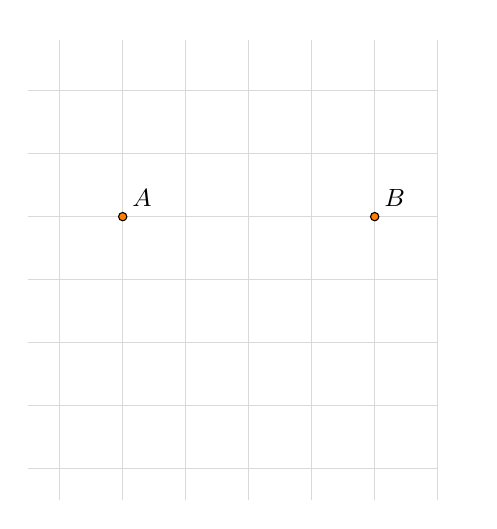
\begin{tikzpicture}[x=8mm, y=8mm,font=\small]

  \node[above right] at (-1,0) {$A$};
  \node[above right] at (3,0) {$B$};
  \draw[step=0.8cm,color=gray!30] (-2.5,-4.5) grid (4,2.8);
  \tkzInit[xmin=-2,xmax=3.5,ymin=-4.5,ymax=2]
  \clip (-2.5,-4.3) rectangle (4.5,3);
  \begin{scope}[font=\small]
    \tkzAxeY[orig = false, label options={left = 1pt}]
    \tkzAxeX[orig = true, label options={below = 1pt}]
  \end{scope}
  \tkzFct[domain=-1.3:3.3,thick,color=Maroon]{x*x-2*x-3};
  \draw[fill=orange] (-1,0)circle (1.5pt);
  \draw[fill=orange] (3,0)circle (1.5pt);

\end{tikzpicture}
% (c) 2012 Dimitrios Vrettos - d.vrettos@gmail.com
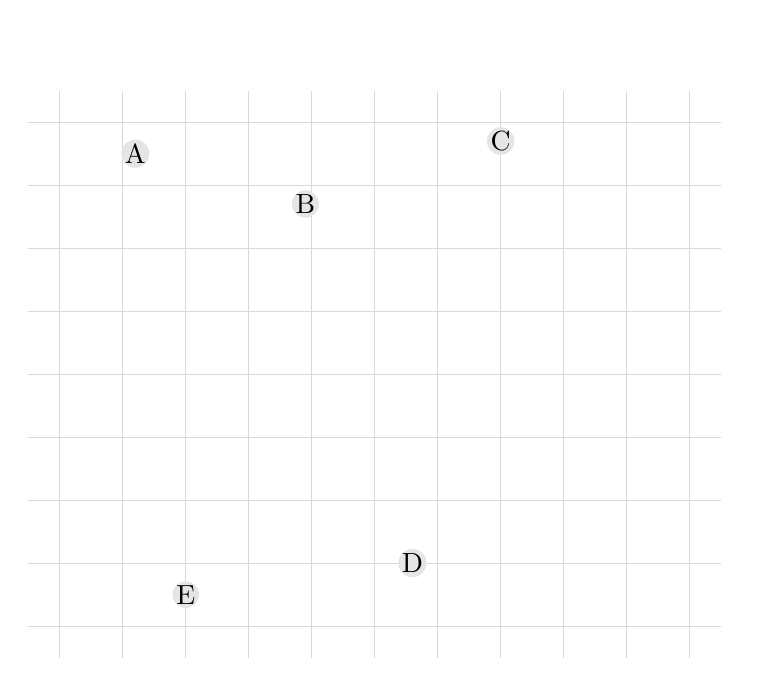
\begin{tikzpicture}[x=8mm, y=8mm]
\draw[step=0.8cm,color=gray!30] (-5.5,-4.5) grid (5.5,4.5);
  \tkzInit[xmin=-5,xmax=5,ymin=-4.5,ymax=4.5]
  \clip (-5.5,-4.5) rectangle (6,5.5);
  \begin{scope}[font=\small]
    \tkzAxeY[orig = false, label options={left = 1pt}]
    \tkzAxeX[orig = true, label options={below = 1pt}]
  \end{scope}
  \tkzFct[domain=-1.5:1.5,thick,color=darkgray]{2*x*x-1}
  \node [inner sep=0pt, circle, fill=gray!20] (a) at (-1.1, 2.7) {B};
  \tkzFct[domain=0:3,thick,color=blue]{-2*x*x+6*x-4};
  \node [inner sep=0pt, circle, fill=gray!20] (a) at (.6, -3) {D};
  \tkzFct[domain=-3.3:-.7,thick,color=RedOrange]{-2*x*x-8*x-8.5};
  \node [inner sep=0pt, circle, fill=gray!20] (a) at (-3, -3.5) {E};
  \tkzFct[domain=1.5:4.5,thick,color=purple]{2*x*x-12*x+18};
  \node [inner sep=0pt, circle, fill=gray!20] (a) at (2, 3.7) {C};
  \tkzFct[domain=-4.5:-1.5,thick,color=olive]{2*x*x+12*x+19};
  \node [inner sep=0pt, circle, fill=gray!20] (a) at (-3.8, 3.5) {A};

\end{tikzpicture}
% (c) 2013 Claudio Carboncini - claudio.carboncini@gmail.com
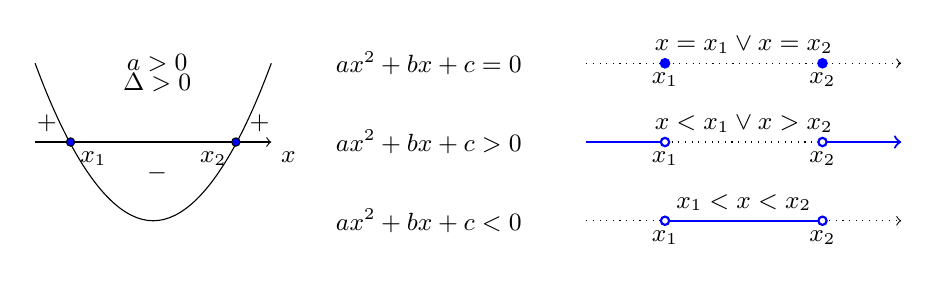
\begin{tikzpicture}[font=\small,x=10mm, y=10mm]

% prima parabola;
  \draw (-1,0) parabola[parabola height=-2cm] +(3,0);
  \draw[->] (-1,-1) -- (2,-1) node [below right] () {$x$};
  \draw[fill=blue] (-.55,-1)circle (1.5pt);
  \draw[fill=blue] (1.55,-1)circle (1.5pt);
  \node[below right] at (-.55,-1) {$x_1$};
  \node[below left] at (1.55,-1) {$x_2$};
  \node[above right] at (1.6,-1) {$+$};
  \node[above left] at (-.6,-1) {$+$};
  \node[] at (.55,-1.4) {$-$};
  \node[] at (.55,-.25) {$\Delta>0$};
  \node[] at (.55,0) {$a>0$};
%segno
  \node[] at (4,0) {$ax^2+bx+c=0$};
  \node[] at (4,-1) {$ax^2+bx+c>0$};
  \node[] at (4,-2) {$ax^2+bx+c<0$};

%Insieme soluzione
%primo insieme
\begin{scope}[dotted]
\draw[->] (6,0) -- (10,0);
\end{scope}
\node[below]  at (7,0) {$x_1$};
\node[below]  at (9,0) {$x_2$};
\node[above]  at (8,0) {$x=x_1 \vee x=x_2$};
\begin{scope}[blue,thick]
\draw[fill=blue] (7,0)circle (1.5pt);
\draw[fill=blue] (9,0)circle (1.5pt);
\end{scope}
%secondo insieme
\begin{scope}[dotted]
\draw (7,-1) -- (9,-1);
\end{scope}
\node[below]  at (7,-1) {$x_1$};
\node[below]  at (9,-1) {$x_2$};
\node[above]  at (8,-1) {$x<x_1 \vee x>x_2$};
\begin{scope}[blue,thick]
\draw (6,-1) -- (7,-1);
\draw[->] (9,-1) -- (10,-1);
\draw[fill=white] (7,-1)circle (1.5pt);
\draw[fill=white] (9,-1)circle (1.5pt);
\end{scope}

%terzo insieme
\begin{scope}[dotted]
\draw (6,-2) -- (7,-2);
\draw[->] (9,-2) -- (10,-2);
\end{scope}
\node[below]  at (7,-2) {$x_1$};
\node[below]  at (9,-2) {$x_2$};
\begin{scope}[blue,thick]
\draw (7,-2) -- (9,-2);
\draw[fill=white] (7,-2)circle (1.5pt);
\draw[fill=white] (9,-2)circle (1.5pt);
\end{scope}
\node[above]  at (8,-2) {$x_1<x<x_2$};

\end{tikzpicture}

% (c) 2013 Claudio Carboncini - claudio.carboncini@gmail.com
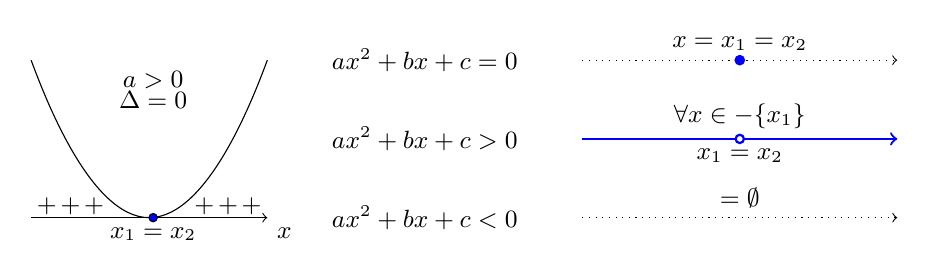
\begin{tikzpicture}[font=\small,x=10mm, y=10mm]

% seconda parabola;
  \draw (-1,0) parabola[parabola height=-2cm] +(3,0);
  \draw[->] (-1,-2) -- (2,-2) node [below right] () {$x$};
  \draw[fill=blue] (.55,-2)circle (1.5pt);
  \foreach \x in {-.8,-.5,-.2,1.2,1.5,1.8}{
  \node  at (\x,-1.85) {$+$};
  }
  \node[below] at (.55,-2) {$x_1=x_2$};
  \node[] at (.55,-.5) {$\Delta=0$};
  \node[] at (.55,-.25) {$a>0$};
%segno
  \node[] at (4,0) {$ax^2+bx+c=0$};
  \node[] at (4,-1) {$ax^2+bx+c>0$};
  \node[] at (4,-2) {$ax^2+bx+c<0$};
%Insieme soluzione

%primo insieme
\begin{scope}[dotted]
\draw (6,0) -- (8,0);
\draw[->] (8,0) -- (10,0);
\end{scope}
\node[above]  at (8,0) {$x=x_1=x_2$};
\begin{scope}[blue,thick]
\draw[fill=blue] (8,0)circle (1.5pt);
\end{scope}

%secondo insieme
\node[below]  at (8,-1) {$x_1=x_2$};
\node[above]  at (8,-1) {$\forall{x} \in \insR-\{x_1\}$};
\begin{scope}[blue,thick]
\draw[->] (6,-1) -- (10,-1);
\draw[fill=white] (8,-1)circle (1.5pt);
\end{scope}

%terzo insieme
\begin{scope}[dotted]
\draw[->] (6,-2) -- (10,-2);
\end{scope}
\node[above]  at (8,-2) {$\IS=\emptyset$};

\end{tikzpicture}

% (c) 2013 Claudio Carboncini - claudio.carboncini@gmail.com
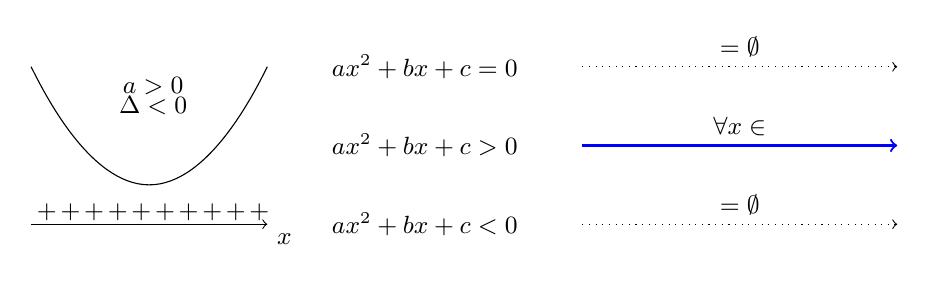
\begin{tikzpicture}[font=\small,x=10mm, y=10mm]

% terza parabola;
  \draw (-1,0) parabola[parabola height=-1.5cm] +(3,0);
  \draw[->] (-1,-2) -- (2,-2) node [below right] () {$x$};
  \foreach \x in {-.8,-.5,-.2,.1,.4,.7,1,1.3,1.6,1.9}{
  \node  at (\x,-1.85) {$+$};
  }
  \node[] at (.55,-.5) {$\Delta<0$};
  \node[] at (.55,-.25) {$a>0$};
%segno
  \node[] at (4,0) {$ax^2+bx+c=0$};
  \node[] at (4,-1) {$ax^2+bx+c>0$};
  \node[] at (4,-2) {$ax^2+bx+c<0$};
%Insieme soluzione
%primo insieme
\begin{scope}[dotted]
\draw[->] (6,0) -- (10,0);
\end{scope}
\node[above]  at (8,0) {$\IS=\emptyset$};
%secondo insieme
\node[above]  at (8,-1) {$\forall x \in \insR$};
\begin{scope}[blue,thick]
\draw[->] (6,-1) -- (10,-1);
\end{scope}
%terzo insieme
\begin{scope}[dotted]
\draw[->] (6,-2) -- (10,-2);
\end{scope}
\node[above]  at (8,-2) {$\IS=\emptyset$};

\end{tikzpicture}

% (c) 2013 Claudio Carboncini - claudio.carboncini@gmail.com
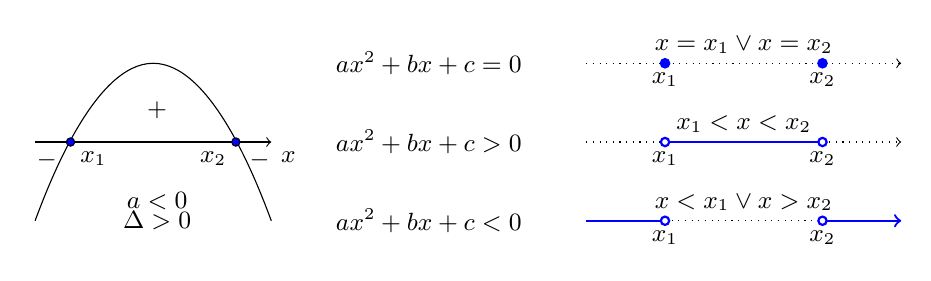
\begin{tikzpicture}[font=\small,x=10mm, y=10mm]

% prima parabola;
  \draw (-1,0) parabola[parabola height=2cm] +(3,0);
  \draw[->] (-1,1) -- (2,1) node [below right] () {$x$};
  \draw[fill=blue] (-.55,1)circle (1.5pt);
  \draw[fill=blue] (1.55,1)circle (1.5pt);
  \node[below right] at (-.55,1) {$x_1$};
  \node[below left] at (1.55,1) {$x_2$};
  \node[below right] at (1.6,1) {$-$};
  \node[below left] at (-.6,1) {$-$};
  \node[] at (.55,1.4) {$+$};
  \node[] at (.55,0) {$\Delta>0$};
  \node[] at (.55,.25) {$a<0$};
%segno
  \node[] at (4,2) {$ax^2+bx+c=0$};
  \node[] at (4,1) {$ax^2+bx+c>0$};
  \node[] at (4,0) {$ax^2+bx+c<0$};

%Insieme soluzione
%primo insieme
\begin{scope}[dotted]
\draw[->] (6,2) -- (10,2);
\end{scope}
\node[below]  at (7,2) {$x_1$};
\node[below]  at (9,2) {$x_2$};
\node[above]  at (8,2) {$x=x_1 \vee x=x_2$};
\begin{scope}[blue,thick]
\draw[fill=blue] (7,2)circle (1.5pt);
\draw[fill=blue] (9,2)circle (1.5pt);
\end{scope}
%secondo insieme
\begin{scope}[dotted]
\draw (6,1) -- (7,1);
\draw[->] (9,1) -- (10,1);
\end{scope}
\node[below]  at (7,1) {$x_1$};
\node[below]  at (9,1) {$x_2$};
\node[above]  at (8,1) {$x_1<x<x_2$};
\begin{scope}[blue,thick]
\draw (7,1) -- (9,1);
\draw[fill=white] (7,1)circle (1.5pt);
\draw[fill=white] (9,1)circle (1.5pt);
\end{scope}

%terzo insieme
\begin{scope}[dotted]
\draw (7,0) -- (9,0);
\end{scope}
\node[below]  at (7,0) {$x_1$};
\node[below]  at (9,0) {$x_2$};
\begin{scope}[blue,thick]
\draw (6,0) -- (7,0);
\draw[->] (9,0) -- (10,0);
\draw[fill=white] (7,0)circle (1.5pt);
\draw[fill=white] (9,0)circle (1.5pt);
\end{scope}
\node[above]  at (8,0) {$x<x_1 \vee x>x_2$};

\end{tikzpicture}

% (c) 2013 Claudio Carboncini - claudio.carboncini@gmail.com
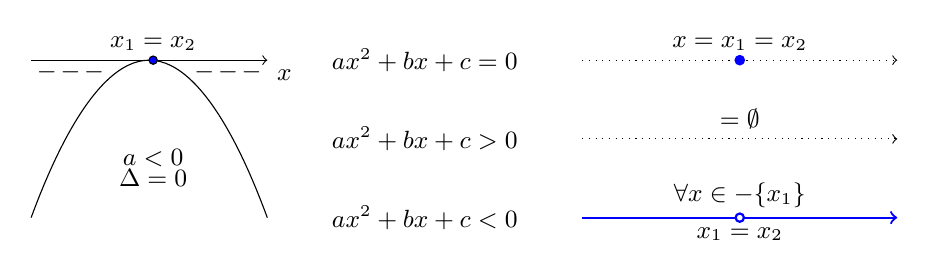
\begin{tikzpicture}[font=\small,x=10mm, y=10mm]

% quarta parabola;
  \draw (-1,0) parabola[parabola height=2cm] +(3,0);
  \draw[->] (-1,2) -- (2,2) node [below right] () {$x$};
  \draw[fill=blue] (.55,2)circle (1.5pt);
  \foreach \x in {-.8,-.5,-.2,1.2,1.5,1.8}{
  \node  at (\x,1.85) {$-$};
  }
  \node[above] at (.55,2) {$x_1=x_2$};
  \node[] at (.55,.5) {$\Delta=0$};
  \node[] at (.55,.75) {$a<0$};
%segno
  \node[] at (4,2) {$ax^2+bx+c=0$};
  \node[] at (4,1) {$ax^2+bx+c>0$};
  \node[] at (4,0) {$ax^2+bx+c<0$};
%Insieme soluzione

%primo insieme
\begin{scope}[dotted]
\draw (6,2) -- (8,2);
\draw[->] (8,2) -- (10,2);
\end{scope}
\node[above]  at (8,2) {$x=x_1=x_2$};
\begin{scope}[blue,thick]
\draw[fill=blue] (8,2)circle (1.5pt);
\end{scope}

%secondo insieme
\begin{scope}[dotted]
\draw[->] (6,1) -- (10,1);
\end{scope}
\node[above]  at (8,1) {$\IS=\emptyset$};

%terzo insieme
\node[below]  at (8,0) {$x_1=x_2$};
\node[above]  at (8,0) {$\forall x \in \insR-\{x_1\}$};
\begin{scope}[blue,thick]
\draw[->] (6,0) -- (10,0);
\draw[fill=white] (8,0)circle (1.5pt);
\end{scope}

\end{tikzpicture}

% (c) 2013 Claudio Carboncini - claudio.carboncini@gmail.com
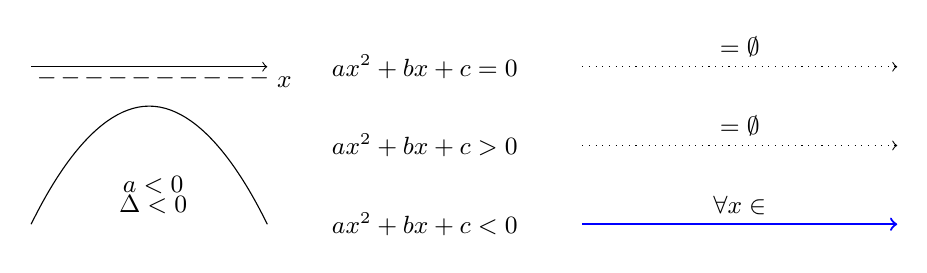
\begin{tikzpicture}[font=\small,x=10mm, y=10mm]

% ultima parabola;
  \draw (-1,0) parabola[parabola height=1.5cm] +(3,0);
  \draw[->] (-1,2) -- (2,2) node [below right] () {$x$};
  \foreach \x in {-.8,-.5,-.2,.1,.4,.7,1,1.3,1.6,1.9}{
    \node  at (\x,1.85) {$-$};
  }
  \node[] at (.55,.25) {$\Delta<0$};
  \node[] at (.55,.5) {$a<0$};
%segno
  \node[] at (4,2) {$ax^2+bx+c=0$};
  \node[] at (4,1) {$ax^2+bx+c>0$};
  \node[] at (4,0) {$ax^2+bx+c<0$};
%Insieme soluzione
%primo insieme
\draw[->, dotted] (6,2) -- (10,2);
\node[above]  at (8,2) {$\IS=\emptyset$};
%secondo insieme
\draw[->, dotted] (6, 1) -- (10, 1);
\node[above]  at (8, 1) {$\IS=\emptyset$};
%terzo insieme
\draw[->, blue,thick] (6, 0) -- (10, 0);
\node[above]  at (8, 0) {$\forall x \in \insR$};

\end{tikzpicture}

% (c) 2013 Claudio Carboncini - claudio.carboncini@gmail.com
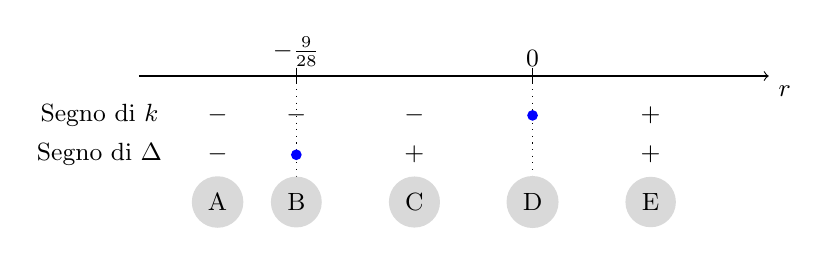
\begin{tikzpicture}[font=\small,x=10mm, y=10mm]

\draw[->] (0,0) -- (8,0) node [below right] () {$r$};

\foreach \x in {2,5}{
\draw(\x,3pt)--(\x,-3pt);
\begin{scope}[dotted]
\draw (\x,0) -- (\x,-1.5);
\end{scope}}
\node[] at (-.5,-0.5) {Segno di $k$};
\node[] at (-.5,-1) {Segno di $\Delta$};
\node[above]  at (2,0) {$-\frac{9}{28}$};
\node[above]  at (5,0) {$0$};
\node[] at (1,-0.5) {$-$};
\node[] at (2,-0.5) {$-$};
\node[] at (3.5,-0.5) {$-$};
\node[] at (6.5,-0.5) {$+$};
\node[] at (1,-1) {$-$};
\node[] at (3.5,-1) {$+$};
\node[] at (6.5,-1) {$+$};
\node [circle,fill=gray!30](A) at (1,-1.6) {A};
\node [circle,fill=gray!30](B) at (2,-1.6) {B};
\node [circle,fill=gray!30](C) at (3.5,-1.6) {C};
\node [circle,fill=gray!30](D) at (5,-1.6) {D};
\node [circle,fill=gray!30](E) at (6.5,-1.6) {E};

\begin{scope}[blue,thick]
\draw[fill=blue] (5,-.5)circle (1.5pt);
\draw[fill=blue] (2,-1)circle (1.5pt);
\end{scope}

\end{tikzpicture}
% (c) 2013 Claudio Carboncini - claudio.carboncini@gmail.com
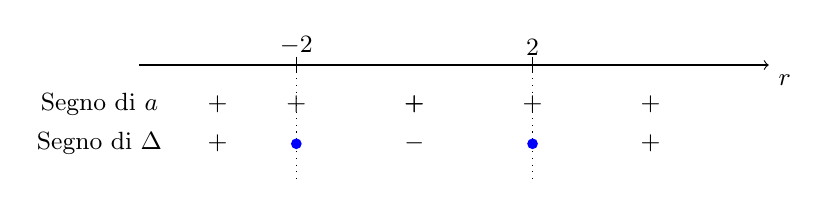
\begin{tikzpicture}[font=\small,x=10mm, y=10mm]

\draw[->] (0,0) -- (8,0) node [below right] () {$r$};

\foreach \x in {2,5}{
\draw(\x,3pt)--(\x,-3pt);
\begin{scope}[dotted]
\draw (\x,0) -- (\x,-1.5);
\end{scope}}
\node[] at (-.5,-0.5) {Segno di $a$};
\node[] at (-.5,-1) {Segno di $\Delta$};
\node[above]  at (2,0) {$-2$};
\node[above]  at (5,0) {$2$};
\node[] at (1,-0.5) {$+$};
\node[] at (2,-0.5) {$+$};
\node[] at (3.5,-0.5) {$+$};
\node[] at (3.5,-0.5) {$+$};
\node[] at (5,-0.5) {$+$};
\node[] at (6.5,-0.5) {$+$};
\node[] at (1,-1) {$+$};
\node[] at (3.5,-1) {$-$};
\node[] at (6.5,-1) {$+$};

\begin{scope}[blue,thick]
\draw[fill=blue] (5,-1)circle (1.5pt);
\draw[fill=blue] (2,-1)circle (1.5pt);
\end{scope}

\end{tikzpicture}
% (c) 2013 Claudio Carboncini - claudio.carboncini@gmail.com
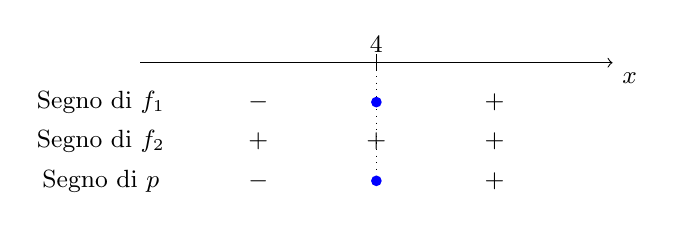
\begin{tikzpicture}[font=\small,x=10mm, y=10mm]

\draw[->] (0,0) -- (6,0) node [below right] () {$x$};

\draw(3,3pt)--(3,-3pt);
\begin{scope}[dotted]
\draw (3,0) -- (3,-1.5);
\end{scope}
\node[] at (-.5,-0.5) {Segno di $f_1$};
\node[] at (-.5,-1) {Segno di $f_2$};
\node[] at (-.5,-1.5) {Segno di $p$};
\node[above]  at (3,0) {$4$};
\node[] at (1.5,-0.5) {$-$};
\node[] at (4.5,-0.5) {$+$};
\node[] at (1.5,-1) {$+$};
\node[] at (3,-1) {$+$};
\node[] at (4.5,-1) {$+$};
\node[] at (1.5,-1.5) {$-$};
\node[] at (4.5,-1.5) {$+$};

\begin{scope}[blue,thick]
\draw[fill=blue] (3,-1.5)circle (1.5pt);
\draw[fill=blue] (3,-.5)circle (1.5pt);
\end{scope}

\end{tikzpicture}
% (c) 2013 Claudio Carboncini - claudio.carboncini@gmail.com
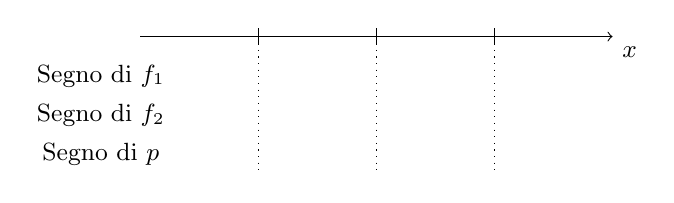
\begin{tikzpicture}[font=\small,x=10mm, y=10mm]

\draw[->] (0,0) -- (6,0) node [below right] () {$x$};

\foreach \x in {1.5,3,4.5}{
\draw(\x,3pt)--(\x,-3pt);
\begin{scope}[dotted]
\draw (\x,0) -- (\x,-1.7);
\end{scope}}
\node[] at (-.5,-0.5) {Segno di $f_1$};
\node[] at (-.5,-1) {Segno di $f_2$};
\node[] at (-.5,-1.5) {Segno di $p$};

\end{tikzpicture}
% (c) 2012 Dimitrios Vrettos - d.vrettos@gmail.com
\begin{tikzpicture}[font=\small,x=10mm, y=10mm]

\matrix (a)[matrix of nodes]{
$\times$& $+$ $-$\\
$+$& $+$ $-$\\
$-$& $-$ $+$\\
};

\begin{scope}[orange]
\draw (a-1-1.north east)--(a-3-1.south east);
\draw (a-1-1.south west)--(a-1-2.south east);
\end{scope}
\end{tikzpicture}% (c) 2012 Dimitrios Vrettos - d.vrettos@gmail.com
\begin{tikzpicture}[font=\small,x=10mm, y=10mm]

\draw[->] (0,0) -- (8,0) node [below right] () {$r$};

\draw(4,3pt)--(4,-3pt);

\node[above]  at (4,0) {$\frac{7}{3}$};

\begin{scope}[blue,thick,->]
\draw (4,0) -- (8,0);
\draw[fill=white] (4,0)circle (1.5pt);
\end{scope}

\end{tikzpicture}% (c) 2013 Claudio Carboncini - claudio.carboncini@gmail.com
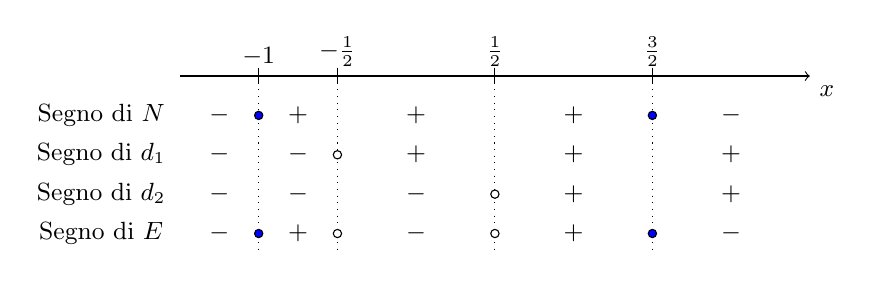
\begin{tikzpicture}[font=\small,x=10mm, y=10mm]

\draw[->] (0,0) -- (8,0) node [below right] () {$x$};

\foreach \x in {1,2,4,6}{
\draw(\x,3pt)--(\x,-3pt);
\begin{scope}[dotted]
\draw (\x,0) -- (\x,-2.2);
\end{scope}}
\node[] at (-1,-0.5) {Segno di $N$};
\draw[fill=blue] (1,-.5)circle (1.5pt);
\draw[fill=blue] (6,-.5)circle (1.5pt);
\node[] at (-1,-1) {Segno di $d_1$};
\draw[fill=white] (2,-1)circle (1.5pt);
\node[] at (-1,-1.5) {Segno di $d_2$};
\draw[fill=white] (4,-1.5)circle (1.5pt);
\node[] at (-1,-2) {Segno di $E$};
\draw[fill=blue] (1,-2)circle (1.5pt);
\draw[fill=blue] (6,-2)circle (1.5pt);
\draw[fill=white] (2,-2)circle (1.5pt);
\draw[fill=white] (4,-2)circle (1.5pt);
\node[above]  at (1,0) {$-1$};
\node[above]  at (2,0) {$-{\frac{1}{2}}$};
\node[above]  at (4,0) {${\frac{1}{2}}$};
\node[above]  at (6,0) {${\frac{3}{2}}$};
\node[] at (.5,-0.5) {$-$};
\node[] at (1.5,-0.5) {$+$};
\node[] at (3,-0.5) {$+$};
\node[] at (5,-0.5) {$+$};
\node[] at (7,-0.5) {$-$};
\node[] at (.5,-1) {$-$};
\node[] at (1.5,-1) {$-$};
\node[] at (3,-1) {$+$};
\node[] at (5,-1) {$+$};
\node[] at (7,-1) {$+$};
\node[] at (.5,-1.5) {$-$};
\node[] at (1.5,-1.5) {$-$};
\node[] at (3,-1.5) {$-$};
\node[] at (5,-1.5) {$+$};
\node[] at (7,-1.5) {$+$};
\node[] at (.5,-2) {$-$};
\node[] at (1.5,-2) {$+$};
\node[] at (3,-2) {$-$};
\node[] at (5,-2) {$+$};
\node[] at (7,-2) {$-$};

\end{tikzpicture}
% (c) 2013 Claudio Carboncini - claudio.carboncini@gmail.com
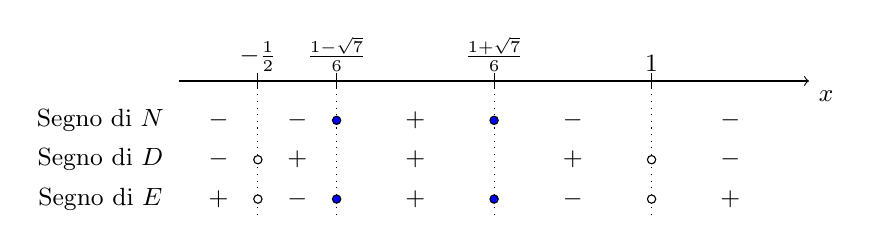
\begin{tikzpicture}[font=\small,x=10mm, y=10mm]

\draw[->] (0,0) -- (8,0) node [below right] () {$x$};

\foreach \x in {1,2,4,6}{
\draw(\x,3pt)--(\x,-3pt);
\begin{scope}[dotted]
\draw (\x,0) -- (\x,-1.7);
\end{scope}}

\node[] at (-1,-0.5) {Segno di $N$};
\draw[fill=blue] (2,-.5)circle (1.5pt);
\draw[fill=blue] (4,-.5)circle (1.5pt);
\node[] at (-1,-1) {Segno di $D$};
\draw[fill=white] (1,-1)circle (1.5pt);
\draw[fill=white] (6,-1)circle (1.5pt);
\node[] at (-1,-1.5) {Segno di $E$};
\draw[fill=blue] (2,-1.5)circle (1.5pt);
\draw[fill=blue] (4,-1.5)circle (1.5pt);
\draw[fill=white] (1,-1.5)circle (1.5pt);
\draw[fill=white] (6,-1.5)circle (1.5pt);
\node[above]  at (1,0) {$-{\frac{1}{2}}$};
\node[above]  at (2,0) {${\frac{1-\sqrt{7}}{6}}$};
\node[above]  at (4,0) {${\frac{1+\sqrt{7}}{6}}$};
\node[above]  at (6,0) {$1$};
\node[] at (.5,-0.5) {$-$};
\node[] at (1.5,-0.5) {$-$};
\node[] at (3,-0.5) {$+$};
\node[] at (5,-0.5) {$-$};
\node[] at (7,-0.5) {$-$};
\node[] at (.5,-1) {$-$};
\node[] at (1.5,-1) {$+$};
\node[] at (3,-1) {$+$};
\node[] at (5,-1) {$+$};
\node[] at (7,-1) {$-$};
\node[] at (.5,-1.5) {$+$};
\node[] at (1.5,-1.5) {$-$};
\node[] at (3,-1.5) {$+$};
\node[] at (5,-1.5) {$-$};
\node[] at (7,-1.5) {$+$};

\end{tikzpicture}
% (c) 2013 Claudio Carboncini - claudio.carboncini@gmail.com
\begin{tikzpicture}[font=\small,x=10mm, y=10mm]

\draw[->] (0,0) -- (8,0) node [below right] () {$r$};

\foreach \x in {2,3.5,5,6.5}{
\draw(\x,3pt)--(\x,-3pt);
\begin{scope}[dotted]
\draw (\x,0) -- (\x,-2);
\draw (0,-.5) -- (2,-.5);
\draw (6.5,-.5) -- (8,-.5);
\draw (3.5,-1) -- (5,-1);
\draw (0,-1.5) -- (2,-1.5);
\draw (3.5,-1.5) -- (5,-1.5);
\draw (6.5,-1.5) -- (8,-1.5);
\end{scope}}

\node[above]  at (2,0) {$\frac{3-2 \sqrt{6}}{3}$};
\node[above]  at (3.5,0) {$\frac{3- \sqrt{5}}{2}$};
\node[above]  at (5,0) {$\frac{3+ \sqrt{5}}{2}$};
\node[above]  at (6.5,0) {$\frac{3+2 \sqrt{6}}{3}$};
\pattern[pattern= north east lines, pattern color=red] (2,-2) rectangle (3.5,-1.5);
\pattern[pattern= north east lines, pattern color=red] (5,-2) rectangle (6.5,-1.5);

\node[] () at (-.5,-.5) {$\IS_{1}$};
\node[] () at (-.5,-1) {$\IS_{2}$};
\node[] () at (-.5,-1.75) {$\IS$};

\begin{scope}[blue,thick]
\draw (2,-.5) -- (6.5,-.5);
\draw (0,-1) -- (3.5,-1);
\draw (5,-1) -- (8,-1);
\draw (2,-1.5) -- (3.5,-1.5);
\draw (5,-1.5) -- (6.5,-1.5);

\draw[fill=blue] (2,-.5)circle (1.5pt);
\draw[fill=blue] (6.5,-.5)circle (1.5pt);
\draw[fill=white] (3.5,-1)circle (1.5pt);
\draw[fill=white] (5,-1)circle (1.5pt);
\draw[fill=blue] (2,-1.5)circle (1.5pt);
\draw[fill=blue] (6.5,-1.5)circle (1.5pt);
\draw[fill=white] (3.5,-1.5)circle (1.5pt);
\draw[fill=white] (5,-1.5)circle (1.5pt);

\end{scope}

\end{tikzpicture}
% (c) 2013 Claudio Carboncini - claudio.carboncini@gmail.com
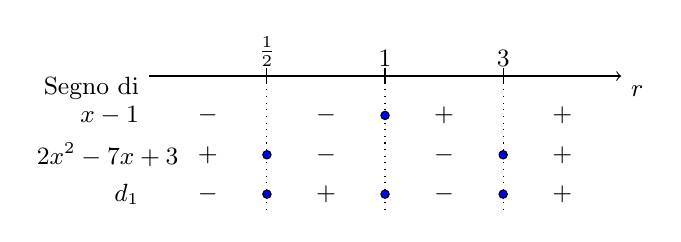
\begin{tikzpicture}[font=\small,x=10mm, y=10mm]

\draw[->] (0,0) -- (6,0) node [below right] () {$r$};

\foreach \x in {1.5,3,4.5}{
\draw(\x,3pt)--(\x,-3pt);
\begin{scope}[dotted]
\draw (\x,0) -- (\x,-1.7);
\end{scope}}

\node[left] at (0,-0.15) {Segno di};
\node[left] at (0,-0.5) {$x-1$};
\node[left] at (.5,-1) {$2x^2-7x+3$};
\node[left] at (0,-1.5) {$d_1$};
\node[above]  at (1.5,0) {$\frac{1}{2}$};
\node[above]  at (3,0) {$1$};
\node[above]  at (4.5,0) {$3$};
\node[] at (.75,-0.5) {$-$};
\node[] at (2.25,-0.5) {$-$};
\node[] at (3.75,-0.5) {$+$};
\node[] at (5.25,-0.5) {$+$};
\node[] at (.75,-1) {$+$};
\node[] at (2.25,-1) {$-$};
\node[] at (3.75,-1) {$-$};
\node[] at (5.25,-1) {$+$};
\node[] at (.75,-1.5) {$-$};
\node[] at (2.25,-1.5) {$+$};
\node[] at (3.75,-1.5) {$-$};
\node[] at (5.25,-1.5) {$+$};

\draw[fill=blue] (3,-.5)circle (1.5pt);
\draw[fill=blue] (1.5,-1)circle (1.5pt);
\draw[fill=blue] (4.5,-1)circle (1.5pt);
\draw[fill=blue] (3,-1.5)circle (1.5pt);
\draw[fill=blue] (1.5,-1.5)circle (1.5pt);
\draw[fill=blue] (4.5,-1.5)circle (1.5pt);

\end{tikzpicture}
% (c) 2013 Claudio Carboncini - claudio.carboncini@gmail.com
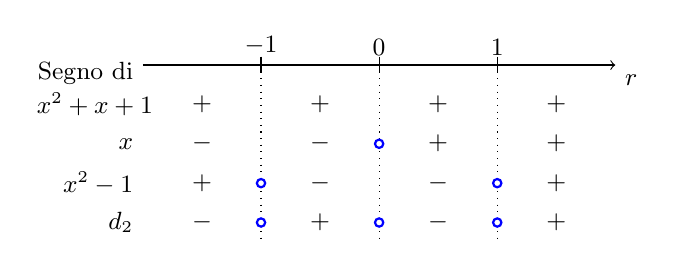
\begin{tikzpicture}[font=\small,x=10mm, y=10mm]

\draw[->] (0,0) -- (6,0) node [below right] () {$r$};

\foreach \x in {1.5,3,4.5}{
\draw(\x,3pt)--(\x,-3pt);
\begin{scope}[dotted]
\draw (\x,0) -- (\x,-2.2);
\end{scope}}

\node[left] at (0,-0.1) {Segno di};
\node[left] at (.25,-0.5) {$x^2+x+1$};
\node[left] at (0,-1) {$x$};
\node[left] at (0,-1.5) {$x^2-1$};
\node[left] at (0,-2) {$d_2$};
\node[above]  at (1.5,0) {$-1$};
\node[above]  at (3,0) {$0$};
\node[above]  at (4.5,0) {$1$};
\node[] at (.75,-0.5) {$+$};
\node[] at (2.25,-0.5) {$+$};
\node[] at (3.75,-0.5) {$+$};
\node[] at (5.25,-0.5) {$+$};
\node[] at (.75,-1) {$-$};
\node[] at (2.25,-1) {$-$};
\node[] at (3.75,-1) {$+$};
\node[] at (5.25,-1) {$+$};
\node[] at (.75,-1.5) {$+$};
\node[] at (2.25,-1.5) {$-$};
\node[] at (3.75,-1.5) {$-$};
\node[] at (5.25,-1.5) {$+$};
\node[] at (.75,-2) {$-$};
\node[] at (2.25,-2) {$+$};
\node[] at (3.75,-2) {$-$};
\node[] at (5.25,-2) {$+$};

\begin{scope}[blue,thick]
\draw[fill=white] (3,-1)circle (1.5pt);
\draw[fill=white] (1.5,-1.5)circle (1.5pt);
\draw[fill=white] (4.5,-1.5)circle (1.5pt);
\draw[fill=white] (3,-2)circle (1.5pt);
\draw[fill=white] (1.5,-2)circle (1.5pt);
\draw[fill=white] (4.5,-2)circle (1.5pt);
\end{scope}

\end{tikzpicture}
% (c) 2013 Claudio Carboncini - claudio.carboncini@gmail.com
\begin{tikzpicture}[font=\small,x=10mm, y=10mm]

\draw[->] (0,0) -- (8,0) node [below right] () {$r$};

\foreach \x in {1,2.3,3.4,4.5,5.6,6.7}{
\draw(\x,3pt)--(\x,-3pt);
\begin{scope}[dotted]
\draw (\x,0) -- (\x,-2.5);
\draw (3.4,-.5) -- (5.6,-.5);
\draw (6.7,-.5) -- (8,-.5);
\draw (0,-1) -- (1,-1);
\draw (2.3,-1) -- (5.6,-1);
\draw (0,-1.5) -- (4.5,-1.5);
\draw (0,-2) -- (5.6,-2);
\draw (6.7,-2) -- (8,-2);
\end{scope}}

\node[above]  at (1,0) {$-1$};
\node[above]  at (2.3,0) {$0$};
\node[above]  at (3.4,0) {$\frac{1}{2}$};
\node[above]  at (4.5,0) {$\frac{3}{4}$};
\node[above]  at (5.6,0) {$1$};
\node[above]  at (6.7,0) {$3$};
\pattern[pattern= north east lines, pattern color=red] (5.6,-2.5) rectangle (6.7,-2);

\node[] () at (-.5,-.5) {$\IS_{1}$};
\node[] () at (-.5,-1) {$\IS_{2}$};
\node[] () at (-.5,-1.5) {$\IS_{3}$};
\node[] () at (-.5,-2.25) {$\IS$};

\begin{scope}[blue,thick]
\draw (0,-.5) -- (3.4,-.5);
\draw (5.6,-.5) -- (6.7,-.5);
\draw (1,-1) -- (2.3,-1);
\draw (5.6,-1) -- (8,-1);
\draw (4.5,-1.5) -- (8,-1.5);
\draw (5.6,-2) -- (6.7,-2);

\draw[fill=blue] (3.4,-.5)circle (1.5pt);
\draw[fill=blue] (5.6,-.5)circle (1.5pt);
\draw[fill=blue] (6.7,-.5)circle (1.5pt);
\draw[fill=white] (1,-1)circle (1.5pt);
\draw[fill=white] (2.3,-1)circle (1.5pt);
\draw[fill=white] (5.6,-1)circle (1.5pt);
\draw[fill=white] (4.5,-1.5)circle (1.5pt);

\draw[fill=white] (5.6,-2)circle (1.5pt);
\draw[fill=blue] (6.7,-2)circle (1.5pt);

\end{scope}

\end{tikzpicture}
% (c) 2014 Daniele Zambelli - daniele.zambelli@gmail.com

%%%
% Retta crescente zero in 2
%%%%
 
\begin{tikzpicture}[x=1.5mm, y=1.5mm, smooth]

% (c) 2014 Daniele Zambelli - daniele.zambelli@gmail.com

%%%
% Retta crescente con segni
%%%%
 
\coordinate (inizio) at (-10, -4);
\coordinate (zero) at (0, 0);
\coordinate (fine) at (10, 4);

% (c) 2014 Daniele Zambelli - daniele.zambelli@gmail.com

%%%
% Asse cartesiano x
%%%%

% (c) 2014 Daniele Zambelli - daniele.zambelli@gmail.com

%%%
% Asse cartesiano generico
%%%%

\draw [-{Stealth[length=2mm, open, round]}] (-10, 0) -- (10, 0);

\node [below] at (10, 0)  {$x$};


\draw [-] [ultra thick, red!50!black] (inizio) -- (zero);
\draw [-] [ultra thick, blue!50!black] (zero) -- (fine);

\node [xshift=-25, yshift=-3, above] at (zero) {$-$};
\draw[blue, thick, fill=white] (zero) circle (2pt);
\node [xshift=25, yshift=-3, above] at (zero) {$+$};

\node [above] {$+2$};

\end{tikzpicture}
% (c) 2014 Daniele Zambelli - daniele.zambelli@gmail.com

%%%
% Retta crescente zero in +2
%%%%
 
\begin{tikzpicture}[x=1.5mm, y=1.5mm, smooth]

% (c) 2014 Daniele Zambelli - daniele.zambelli@gmail.com

%%%
% Retta crescente con segni
%%%%
 
\coordinate (inizio) at (-10, -4);
\coordinate (zero) at (0, 0);
\coordinate (fine) at (10, 4);

% (c) 2014 Daniele Zambelli - daniele.zambelli@gmail.com

%%%
% Asse cartesiano x
%%%%

% (c) 2014 Daniele Zambelli - daniele.zambelli@gmail.com

%%%
% Asse cartesiano generico
%%%%

\draw [-{Stealth[length=2mm, open, round]}] (-10, 0) -- (10, 0);

\node [below] at (10, 0)  {$x$};


\draw [-] [ultra thick, red!50!black] (inizio) -- (zero);
\draw [-] [ultra thick, blue!50!black] (zero) -- (fine);

\node [xshift=-25, yshift=-3, above] at (zero) {$-$};
\draw[blue, thick, fill=white] (zero) circle (2pt);
\node [xshift=25, yshift=-3, above] at (zero) {$+$};

\node [above] {$-2$};

\end{tikzpicture}
% (c) 2014 Daniele Zambelli - daniele.zambelli@gmail.com

%%%
% Retta decrescente zero in 1/2
%%%%
 
\begin{tikzpicture}[x=1.5mm, y=1.5mm, smooth]

% (c) 2014 Daniele Zambelli - daniele.zambelli@gmail.com

%%%
% Retta decrescente con segni
%%%%
 
\coordinate (inizio) at (-10, 4);
\coordinate (zero) at (0, 0);
\coordinate (fine) at (10, -4);

% (c) 2014 Daniele Zambelli - daniele.zambelli@gmail.com

%%%
% Asse cartesiano x
%%%%

% (c) 2014 Daniele Zambelli - daniele.zambelli@gmail.com

%%%
% Asse cartesiano generico
%%%%

\draw [-{Stealth[length=2mm, open, round]}] (-10, 0) -- (10, 0);

\node [below] at (10, 0)  {$x$};


\draw [-] [ultra thick, blue!50!black] (inizio) -- (zero);
\draw [-] [ultra thick, red!50!black] (zero) -- (fine);

\node [xshift=-25, yshift=-3, above] at (zero) {$+$};
\draw[blue, thick, fill=white] (zero) circle (2pt);
\node [xshift=25, yshift=-3, above] at (zero) {$-$};

\node [above] {$\frac{3}{2}$};

\end{tikzpicture}
% (c) 2014 Daniele Zambelli - daniele.zambelli@gmail.com

%%%
% Retta decrescente zero in 3
%%%%
 
\begin{tikzpicture}[x=1.5mm, y=1.5mm, smooth]

% (c) 2014 Daniele Zambelli - daniele.zambelli@gmail.com

%%%
% Retta decrescente con segni
%%%%
 
\coordinate (inizio) at (-10, 4);
\coordinate (zero) at (0, 0);
\coordinate (fine) at (10, -4);

% (c) 2014 Daniele Zambelli - daniele.zambelli@gmail.com

%%%
% Asse cartesiano x
%%%%

% (c) 2014 Daniele Zambelli - daniele.zambelli@gmail.com

%%%
% Asse cartesiano generico
%%%%

\draw [-{Stealth[length=2mm, open, round]}] (-10, 0) -- (10, 0);

\node [below] at (10, 0)  {$x$};


\draw [-] [ultra thick, blue!50!black] (inizio) -- (zero);
\draw [-] [ultra thick, red!50!black] (zero) -- (fine);

\node [xshift=-25, yshift=-3, above] at (zero) {$+$};
\draw[blue, thick, fill=white] (zero) circle (2pt);
\node [xshift=25, yshift=-3, above] at (zero) {$-$};

\node [above] {$+29$};

\end{tikzpicture}
% (c) 2014 Daniele Zambelli - daniele.zambelli@gmail.com

%%%
% Retta crescente zero in -2
%%%%
 
\begin{tikzpicture}[x=1.5mm, y=1.5mm, smooth]

% (c) 2014 Daniele Zambelli - daniele.zambelli@gmail.com

%%%
% Retta crescente con segni
%%%%
 
\coordinate (inizio) at (-10, -4);
\coordinate (zero) at (0, 0);
\coordinate (fine) at (10, 4);

% (c) 2014 Daniele Zambelli - daniele.zambelli@gmail.com

%%%
% Asse cartesiano x
%%%%

% (c) 2014 Daniele Zambelli - daniele.zambelli@gmail.com

%%%
% Asse cartesiano generico
%%%%

\draw [-{Stealth[length=2mm, open, round]}] (-10, 0) -- (10, 0);

\node [below] at (10, 0)  {$x$};


\draw [-] [ultra thick, red!50!black] (inizio) -- (zero);
\draw [-] [ultra thick, blue!50!black] (zero) -- (fine);

\node [xshift=-25, yshift=-3, above] at (zero) {$-$};
\draw[blue, thick, fill=white] (zero) circle (2pt);
\node [xshift=25, yshift=-3, above] at (zero) {$+$};

\node [above] {$+7$};

\end{tikzpicture}
% (c) 2014 Daniele Zambelli - daniele.zambelli@gmail.com

%%%
% Retta crescente zero in -2
%%%%
 
\begin{tikzpicture}[x=1.5mm, y=1.5mm, smooth]

% (c) 2014 Daniele Zambelli - daniele.zambelli@gmail.com

%%%
% Retta crescente con segni
%%%%
 
\coordinate (inizio) at (-10, -4);
\coordinate (zero) at (0, 0);
\coordinate (fine) at (10, 4);

% (c) 2014 Daniele Zambelli - daniele.zambelli@gmail.com

%%%
% Asse cartesiano x
%%%%

% (c) 2014 Daniele Zambelli - daniele.zambelli@gmail.com

%%%
% Asse cartesiano generico
%%%%

\draw [-{Stealth[length=2mm, open, round]}] (-10, 0) -- (10, 0);

\node [below] at (10, 0)  {$x$};


\draw [-] [ultra thick, red!50!black] (inizio) -- (zero);
\draw [-] [ultra thick, blue!50!black] (zero) -- (fine);

\node [xshift=-25, yshift=-3, above] at (zero) {$-$};
\draw[blue, thick, fill=white] (zero) circle (2pt);
\node [xshift=25, yshift=-3, above] at (zero) {$+$};

\node [above] {$-4$};

\end{tikzpicture}
% (c) 2014 Daniele Zambelli - daniele.zambelli@gmail.com

%%%
% Studio dei segni di una frazione
%%%%
 
\begin{tikzpicture}[x=2.5mm, y=5mm, smooth]

\coordinate (a_top) at (-5, 1);
\coordinate (a_bottom) at (-5, -3);
\coordinate (b_top) at (0, 1);
\coordinate (b_bottom) at (0, -3);
\coordinate (c_top) at (5, 1);
\coordinate (c_bottom) at (5, -3);

% (c) 2014 Daniele Zambelli - daniele.zambelli@gmail.com

%%%
% Grafo per il calcolo del segno con tre assi
%%%%
 
% (c) 2014 Daniele Zambelli - daniele.zambelli@gmail.com

%%%
% Asse cartesiano x
%%%%

% (c) 2014 Daniele Zambelli - daniele.zambelli@gmail.com

%%%
% Asse cartesiano generico
%%%%

\draw [-{Stealth[length=2mm, open, round]}] (-10, 0) -- (10, 0);

\node [below] at (10, 0)  {$x$};

\begin{scope}[yshift= -.5cm]
  % (c) 2014 Daniele Zambelli - daniele.zambelli@gmail.com

%%%
% Asse cartesiano x
%%%%

% (c) 2014 Daniele Zambelli - daniele.zambelli@gmail.com

%%%
% Asse cartesiano generico
%%%%

\draw [-{Stealth[length=2mm, open, round]}] (-10, 0) -- (10, 0);

\node [below] at (10, 0)  {$x$};

  \begin{scope}[yshift= -.5cm]
    % (c) 2014 Daniele Zambelli - daniele.zambelli@gmail.com

%%%
% Asse cartesiano x
%%%%

% (c) 2014 Daniele Zambelli - daniele.zambelli@gmail.com

%%%
% Asse cartesiano generico
%%%%

\draw [-{Stealth[length=2mm, open, round]}] (-10, 0) -- (10, 0);

\node [below] at (10, 0)  {$x$};

    \begin{scope}[yshift= -.5cm]
      % (c) 2014 Daniele Zambelli - daniele.zambelli@gmail.com

%%%
% Asse cartesiano x
%%%%

% (c) 2014 Daniele Zambelli - daniele.zambelli@gmail.com

%%%
% Asse cartesiano generico
%%%%

\draw [-{Stealth[length=2mm, open, round]}] (-10, 0) -- (10, 0);

\node [below] at (10, 0)  {$x$};

    \end{scope}
  \end{scope}
\end{scope}

\draw [-] [] (a_top) -- (a_bottom);
\draw [-] [] (b_top) -- (b_bottom);
\draw [-] [] (c_top) -- (c_bottom);

\node [above] at (-5, 1) {$-4$};
\node [above] at (0, 1) {$+7$};
\node [above] at (5, 1) {$+29$};

\node [above left] at (-10, 0) {$-x+29$};
\node [above] at (-7.5, 0) {$+$};
\node [above] at (-2.5, 0) {$+$};
\node [above] at (2.5, 0) {$+$};
\draw (5, .5) circle (3pt);
\node [above] at (7.5, 0) {$-$};

\node [above left] at (-10, -1) {$x-7$};
\node [above] at (-7.5, -1) {$-$};
\node [above] at (-2.5, -1) {$-$};
\draw (0 -.4, -0.5 -.2) -- (0 +.4, -0.5 +.2) 
      (0 -.4, -0.5 +.2) -- (0 +.4, -0.5 -.2);
\node [above] at (2.5, -1) {$+$};
\node [above] at (7.5, -1) {$+$};

\node [above left] at (-10, -2) {$x+4$};
\node [above] at (-7.5, -2) {$-$};
\draw (-5 -.4, -1.5 -.2) -- (-5 +.4, -1.5 +.2) 
      (-5 -.4, -1.5 +.2) -- (-5 +.4, -1.5 -.2);
\node [above] at (-2.5, -2) {$+$};
\node [above] at (2.5, -2) {$+$};
\node [above] at (7.5, -2) {$+$};

\node [above left] at (-10, -3.15) {$F(x)$};
\node [above] at (-7.5, -3) {$+$};
\draw (-5 -.4, -2.5 -.2) -- (-5 +.4, -2.5 +.2) 
      (-5 -.4, -2.5 +.2) -- (-5 +.4, -2.5 -.2);
\node [above] at (-2.5, -3) {$-$};
\draw (0 -.4, -2.5 -.2) -- (0 +.4, -2.5 +.2) 
      (0 -.4, -2.5 +.2) -- (0 +.4, -2.5 -.2);
\node [above] at (2.5, -3) {$+$};
\draw (5, -2.5) circle (3pt);
\node [above] at (7.5, -3) {$-$};

\end{tikzpicture}
% (c) 2014 Daniele Zambelli - daniele.zambelli@gmail.com

%%%
% Valori x < -4  or  7 < x <= 29
%%%%
 
\begin{tikzpicture}[x=1.5mm, y=1.5mm, smooth]

% \clip (-7.5, -5.5) rectangle (10.9, 10.9);

\coordinate (m_i) at (-10, 0);
\coordinate (a) at (-5, 0);
\coordinate (b) at (0, 0);
\coordinate (c) at (5, 0);
\coordinate (p_i) at (10, 0);

% (c) 2014 Daniele Zambelli - daniele.zambelli@gmail.com

%%%
% Asse cartesiano x
%%%%

% (c) 2014 Daniele Zambelli - daniele.zambelli@gmail.com

%%%
% Asse cartesiano generico
%%%%

\draw [-{Stealth[length=2mm, open, round]}] (-10, 0) -- (10, 0);

\node [below] at (10, 0)  {$x$};


\begin{scope}[blue,thick]
\draw [-,decorate,decoration=snake] (m_i) -- (a);
% \draw[fill=white] (a) circle (2pt) node [above] {$-3$};
\draw[fill=white] (a) circle (2pt) node [above] {$-4$};
% \draw [-,decorate,decoration=snake] (b) -- (c);
\draw[fill=white] (b) circle (2pt) node [above] {$+7$};
\draw [decorate,decoration=snake] (b) -- (c);
\draw[fill] (c) circle (2pt) node [above] {$+29$};
\end{scope}

\end{tikzpicture}
% (c) 2014 Daniele Zambelli - daniele.zambelli@gmail.com

%%%
% Grafo per il calcolo del segno con tre assi
%%%%
 
% (c) 2014 Daniele Zambelli - daniele.zambelli@gmail.com

%%%
% Asse cartesiano x
%%%%

% (c) 2014 Daniele Zambelli - daniele.zambelli@gmail.com

%%%
% Asse cartesiano generico
%%%%

\draw [-{Stealth[length=2mm, open, round]}] (-10, 0) -- (10, 0);

\node [below] at (10, 0)  {$x$};

\begin{scope}[yshift= -.5cm]
  % (c) 2014 Daniele Zambelli - daniele.zambelli@gmail.com

%%%
% Asse cartesiano x
%%%%

% (c) 2014 Daniele Zambelli - daniele.zambelli@gmail.com

%%%
% Asse cartesiano generico
%%%%

\draw [-{Stealth[length=2mm, open, round]}] (-10, 0) -- (10, 0);

\node [below] at (10, 0)  {$x$};

  \begin{scope}[yshift= -.5cm]
    % (c) 2014 Daniele Zambelli - daniele.zambelli@gmail.com

%%%
% Asse cartesiano x
%%%%

% (c) 2014 Daniele Zambelli - daniele.zambelli@gmail.com

%%%
% Asse cartesiano generico
%%%%

\draw [-{Stealth[length=2mm, open, round]}] (-10, 0) -- (10, 0);

\node [below] at (10, 0)  {$x$};

    \begin{scope}[yshift= -.5cm]
      % (c) 2014 Daniele Zambelli - daniele.zambelli@gmail.com

%%%
% Asse cartesiano x
%%%%

% (c) 2014 Daniele Zambelli - daniele.zambelli@gmail.com

%%%
% Asse cartesiano generico
%%%%

\draw [-{Stealth[length=2mm, open, round]}] (-10, 0) -- (10, 0);

\node [below] at (10, 0)  {$x$};

    \end{scope}
  \end{scope}
\end{scope}

\draw [-] [] (a_top) -- (a_bottom);
\draw [-] [] (b_top) -- (b_bottom);
\draw [-] [] (c_top) -- (c_bottom);
% (c) 2014 Daniele Zambelli - daniele.zambelli@gmail.com

%%%
% Retta crescente con segni
%%%%
 
\coordinate (inizio) at (-10, -4);
\coordinate (zero) at (0, 0);
\coordinate (fine) at (10, 4);

% (c) 2014 Daniele Zambelli - daniele.zambelli@gmail.com

%%%
% Asse cartesiano x
%%%%

% (c) 2014 Daniele Zambelli - daniele.zambelli@gmail.com

%%%
% Asse cartesiano generico
%%%%

\draw [-{Stealth[length=2mm, open, round]}] (-10, 0) -- (10, 0);

\node [below] at (10, 0)  {$x$};


\draw [-] [ultra thick, red!50!black] (inizio) -- (zero);
\draw [-] [ultra thick, blue!50!black] (zero) -- (fine);

\node [xshift=-25, yshift=-3, above] at (zero) {$-$};
\draw[blue, thick, fill=white] (zero) circle (2pt);
\node [xshift=25, yshift=-3, above] at (zero) {$+$};
% (c) 2014 Daniele Zambelli - daniele.zambelli@gmail.com

%%%
% Retta decrescente con segni
%%%%
 
\coordinate (inizio) at (-10, 4);
\coordinate (zero) at (0, 0);
\coordinate (fine) at (10, -4);

% (c) 2014 Daniele Zambelli - daniele.zambelli@gmail.com

%%%
% Asse cartesiano x
%%%%

% (c) 2014 Daniele Zambelli - daniele.zambelli@gmail.com

%%%
% Asse cartesiano generico
%%%%

\draw [-{Stealth[length=2mm, open, round]}] (-10, 0) -- (10, 0);

\node [below] at (10, 0)  {$x$};


\draw [-] [ultra thick, blue!50!black] (inizio) -- (zero);
\draw [-] [ultra thick, red!50!black] (zero) -- (fine);

\node [xshift=-25, yshift=-3, above] at (zero) {$+$};
\draw[blue, thick, fill=white] (zero) circle (2pt);
\node [xshift=25, yshift=-3, above] at (zero) {$-$};

\end{comment}